%%%%%%%%%%%%%%%%%%%%%%%%%%%%%%%%%%%%%%%%%%%%%%%%%%%
%
%  New template code for TAMU Theses and Dissertations starting Fall 2012.  
%  For more info about this template or the 
%  TAMU LaTeX User's Group, see http://www.howdy.me/.
%
%  Author: Wendy Lynn Turner 
%
%%%%%%%%%%%%%%%%%%%%%%%%%%%%%%%%%%%%%%%%%%%%%%%%%%%

\documentclass[12pt]{report}
\usepackage[letterpaper]{geometry}
\geometry{verbose,tmargin=1.25in,bmargin=1.25in,lmargin=1.4in,rmargin=1.15in}
 \usepackage[doublespacing]{setspace}
 \usepackage{tocloft}
 \usepackage[rm, tiny,center, compact]{titlesec}
 \usepackage{indentfirst}
 \usepackage{etoolbox}
\usepackage{tocvsec2}
 \usepackage[titletoc]{appendix}
 \usepackage{appendix}
 \usepackage{tamuconfig}
\usepackage{rotating}
\usepackage{amsmath}
\usepackage{graphicx}
\usepackage{subcaption}
\usepackage{tabularx}
%\usepackage{breqn}
\usepackage[linesnumbered,lined,boxed,commentsnumbered]{algorithm2e}
\allowdisplaybreaks

\makeatletter
\renewcommand{\@biblabel}[1]{[#1]\hfill}
\makeatother
% Added to fix issues with pdf searching in some versions of LaTeX
%\usepackage[T1]{fontenc}\usepackage{lmodern}
%%%%%%%%%%%%%%%%%%%%%%%%%%%%%

% Hyperref setup below.  You should be able to get away with using uncommenting just the first line.
\usepackage[hidelinks]{hyperref}

% if \usepackage[hidelinks]{hyperref} doesn't work try this.
% \usepackage{hyperref}  % Hidelinks is an option that removes link visiability.  TAMU Thesis Offices prefers to not see the links. But often doesn't work.  
% 
% \hypersetup{
%     colorlinks=true,
%     linkcolor=black,
%     citecolor=black,
%     filecolor=black,
%     urlcolor=black,
% }
%%%%%%%  End of hyperref setup.  One of these two options should work, but my motto with hyperref is when in doubt, comment it out!
%%%%%%%%%  This hopefully fixes the problem with vertical spacing of section headings at the top of the page..  Commented out in 1.0.7
% \preto\section{%
% \ifnum\value{section}>0\addtocontents{toc}{\vskip-6pt}\fi
% }
% \preto\subsection{%
% \ifnum\value{subsection}=0\addtocontents{toc}{\vskip-6pt}\fi
% \ifnum\value{subsection}>0\addtocontents{toc}{\vskip-6pt}\fi
% } 
%%%%%%%%%%%%%%%%%%%%%%%%%%%%%%%%%%%%%%%%%%%%%%%%%%%%%%

\begin{document}

\renewcommand{\tamumanuscripttitle}{Type in your default title here: You may need to change the spacing if the title is too long and pushes the copyright off of the titlepage }
\renewcommand{\tamupapertype}{Dissertation}
\renewcommand{\tamufullname}{First Middle Lastname}
\renewcommand{\tamudegree}{Doctor of Philosophy}
\renewcommand{\tamuchairone}{Chair Name}
% Uncomment out the next line if you have co-chairs.  You will also need to edit the titlepage.tex file.
%\newcommand{\tamuchairtwo}{Additional Chair Name}
\renewcommand{\tamumemberone}{Committee Member1}
\newcommand{\tamumembertwo}{Committee Member2}
\newcommand{\tamumemberthree}{Committee Member3}
\renewcommand{\tamudepthead}{Head of Department}
\renewcommand{\tamugradmonth}{December}
\renewcommand{\tamugradyear}{2012}
\renewcommand{\tamudepartment}{Department Name}


%%%%%%%%%%%%%%%%%%%%%%%%%%%%%%%%%%%%%%%%%%%%%%%%%%%
%
%  New template code for TAMU Theses and Dissertations starting Fall 2012.  
%  For more info about this template or the 
%  TAMU LaTeX User's Group, see http://www.howdy.me/.
%
%  Author: Wendy Lynn Turner 
%	 Version 1.0 
%  Last updated 8/5/2012
%
%%%%%%%%%%%%%%%%%%%%%%%%%%%%%%%%%%%%%%%%%%%%%%%%%%%

%%%%%%%%%%%%%%%%%%%%%%%%%%%%%% 
%% TITLE PAGE
%% The values get updated automatically.  Please do not make changes to this file other than adding/deleting committee members where necessary.
%%%%%%%%%%%%%%%%%%%%%%%%%%%%%%

\providecommand{\tabularnewline}{\\}



\begin{titlepage}
\begin{center}
\MakeUppercase{\tamumanuscripttitle}
\vspace{4em}

A \tamupapertype

by

\MakeUppercase{\tamufullname}

\vspace{4em}

\begin{singlespace}

Submitted to the Office of Graduate and Professional Studies of \\
Texas A\&M University \\

in partial fulfillment of the requirements for the degree of \\
\end{singlespace}

\MakeUppercase{\tamudegree}
\par\end{center}
\vspace{2em}
\begin{singlespace}
\begin{tabular}{ll}
 & \tabularnewline
& \cr
% If you have Co-Chairs comment out the 'Chair of Committee' line below and uncomment the 'Co-Chairs of Committee' line.
Chair of Committee, & \tamuchairone\tabularnewline
%Co-Chairs of Committee, & \tamuchairone\tabularnewline & \tamuchairtwo\tabularnewline
Committee Members, & \tamumemberone\tabularnewline
 & \tamumembertwo\tabularnewline
 & \tamumemberthree\tabularnewline
Head of Department, & \tamudepthead\tabularnewline

\end{tabular}
\end{singlespace}
\vspace{3em}

\begin{center}
\tamugradmonth \hspace{2pt} \tamugradyear

\vspace{3em}

Major Subject: \tamudepartment \par
\vspace{3em}
Copyright \tamugradyear \hspace{.5em}\tamufullname 
\par\end{center}
\end{titlepage}
\pagebreak{}




 % This is simply a file that formats and adds your titlepage, please do not edit this unless you have a specific need. .
%%%%%%%%%%%%%%%%%%%%%%%%%%%%%%%%%%%%%%%%%%%%%%%%%%%
%
%  New template code for TAMU Theses and Dissertations starting Fall 2012.  
%  For more info about this template or the 
%  TAMU LaTeX User's Group, see http://www.howdy.me/.
%
%  Author: Wendy Lynn Turner 
%	 Version 1.0 
%  Last updated 8/5/2012
%
%%%%%%%%%%%%%%%%%%%%%%%%%%%%%%%%%%%%%%%%%%%%%%%%%%%
%%%%%%%%%%%%%%%%%%%%%%%%%%%%%%%%%%%%%%%%%%%%%%%%%%%%%%%%%%%%%%%%%%%%%
%%                           ABSTRACT 
%%%%%%%%%%%%%%%%%%%%%%%%%%%%%%%%%%%%%%%%%%%%%%%%%%%%%%%%%%%%%%%%%%%%%

\chapter*{ABSTRACT}
\addcontentsline{toc}{chapter}{ABSTRACT} % Needs to be set to part, so the TOC doesnt add 'CHAPTER ' prefix in the TOC.

\pagestyle{plain} % No headers, just page numbers
\pagenumbering{roman} % Roman numerals
\setcounter{page}{2}

\indent Lorem ipsum dolor sit amet, consectetur adipiscing elit. Integer lectus quam, condimentum quis bibendum eu, sollicitudin eget lacus. Praesent non sodales odio. Class aptent taciti sociosqu ad litora torquent per conubia nostra, per inceptos himenaeos. Nulla ac luctus sapien. Morbi cursus sapien eget lorem fermentum hendrerit. Nam ac erat dui, in cursus velit. Vivamus hendrerit porttitor nisi, ut porttitor lorem volutpat eget. In ligula ligula, euismod ut condimentum sit amet, pulvinar sit amet diam. Pellentesque interdum, ipsum ullamcorper consequat dignissim, sem arcu egestas mauris, vitae interdum sem tortor ut ante. Nunc blandit laoreet nisi, non rutrum lorem hendrerit quis. Cras nunc diam, convallis et feugiat at, auctor id libero. Nunc facilisis massa eu eros imperdiet vestibulum. Vestibulum ante ipsum primis in faucibus orci luctus et ultrices posuere cubilia Curae; Donec non velit vitae tortor blandit semper.

Etiam vitae dolor nulla. Ut eros odio, rhoncus eget placerat vitae, elementum ac ante. Proin vitae odio eu nisl pharetra mattis. Pellentesque habitant morbi tristique senectus et netus et malesuada fames ac turpis egestas. Phasellus fermentum lacus consectetur neque consequat ullamcorper. Cras blandit urna non dui consequat molestie. Curabitur viverra nibh at nisi semper faucibus. Nam egestas mauris a enim dignissim nec consectetur tortor rutrum. Mauris at nisi in est luctus congue ut mattis est. Ut pretium, mi quis elementum cursus, ante eros suscipit ligula, ut porttitor elit leo sed turpis. Nam sed dui ligula.

 

\pagebreak{}

%%%%%%%%%%%%%%%%%%%%%%%%%%%%%%%%%%%%%%%%%%%%%%%%%%%
%
%  New template code for TAMU Theses and Dissertations starting Fall 2012.  
%  For more info about this template or the 
%  TAMU LaTeX User's Group, see http://www.howdy.me/.
%
%  Author: Wendy Lynn Turner 
%	 Version 1.0 
%  Last updated 8/5/2012
%
%%%%%%%%%%%%%%%%%%%%%%%%%%%%%%%%%%%%%%%%%%%%%%%%%%%

%%%%%%%%%%%%%%%%%%%%%%%%%%%%%%%%%%%%%%%%%%%%%%%%%%%%%%%%%%%%%%%%%%%%%%
%%                           DEDICATION
%%%%%%%%%%%%%%%%%%%%%%%%%%%%%%%%%%%%%%%%%%%%%%%%%%%%%%%%%%%%%%%%%%%%%
\chapter*{}
%\addcontentsline{toc}{chapter}{EPIGRAPH}  % Needs to be set to part, so the TOC doesnt add 'CHAPTER ' prefix in the TOC.


\begin{displayquote}
``To live is to suffer, to survive is to find some meaning in the suffering.''
\end{displayquote}
\hspace{4 in}--Friedrich Nietzsche%Taylor Swift
%aFriedrich Nietzsche

\pagebreak{}

%%%%%%%%%%%%%%%%%%%%%%%%%%%%%%%%%%%%%%%%%%%%%%%%%%%
%
%  New template code for TAMU Theses and Dissertations starting Fall 2012.  
%  For more info about this template or the 
%  TAMU LaTeX User's Group, see http://www.howdy.me/.
%
%  Author: Wendy Lynn Turner 
%	 Version 1.0 
%  Last updated 8/5/2012
%
%%%%%%%%%%%%%%%%%%%%%%%%%%%%%%%%%%%%%%%%%%%%%%%%%%%


%%%%%%%%%%%%%%%%%%%%%%%%%%%%%%%%%%%%%%%%%%%%%%%%%%%%%%%%%%%%%%%%%%%%%%
%%                           ACKNOWLEDGEMENTS
%%%%%%%%%%%%%%%%%%%%%%%%%%%%%%%%%%%%%%%%%%%%%%%%%%%%%%%%%%%%%%%%%%%%%
\chapter*{ACKNOWLEDGEMENTS}
\addcontentsline{toc}{chapter}{ACKNOWLEDGEMENTS}  % Needs to be set to part, so the TOC doesnt add 'CHAPTER ' prefix in the TOC.

Starting with the obvious, I would like to express my gratitude to Dr. Jim Morel for your guidance and 
willingness to impart your transport wisdom on me over the last few years.  In addition to being a prime source of
knowledge, as an advisor you seem to find the appropriate balance between blind patience and hard-nosed
motivation, where the focus is always exclusively on the problem under investigation.
 I would also like to thank Dr. McClarren and Dr. Ragusa for always willingly providing
alternative view points and discussion on interesting topics, often unrelated to work and
occasionally involving fine beverages. Overall, it has been a pleasure being part of this research group. 

 I would like to thank my parents for a great childhood and continued support, as well
as for never pressuring me to get a real job or take over the farm\ldots yet.  And of course my friends
at A\&M deserve credit for the constant antics and shenanigans that help take the edge off of grad
school.  I must also acknowledge my friend Hank; I cannot imagine my life would have
went down this academic path if we hadn't met.  And finally, I would like to thank my (now) wife Madeline.  I think it goes without much
explanation, but you have always been easy-going through this process and made life pleasant.

Finally, I would like to acknowledge the financial and educational support I have received
over the years. This research was supported with funding received from the DOE Office of Nuclear
Energy's Nuclear Energy University Programs, the DOE National
Nuclear Security Administration, under Award Number(s) DE-NA0002376, and under Los Alamos National Security,
LLC, for the National Nuclear Security Administration of the U.S. Department of
Energy under contract DE-AC52-06NA25396. 

%%%%%%%%%%%%%%%%%%%%%%%%%%%%%%%%%%%%%%%%%%%%%%%%%%%
%
%  New template code for TAMU Theses and Dissertations starting Fall 2012.  
%  For more info about this template or the 
%  TAMU LaTeX User's Group, see http://www.howdy.me/.
%
%  Author: Wendy Lynn Turner 
%	 Version 1.0 
%  Last updated 8/5/2012
%
%%%%%%%%%%%%%%%%%%%%%%%%%%%%%%%%%%%%%%%%%%%%%%%%%%%

%%%%%%%%%%%%%%%%%%%%%%%%%%%%%%%%%%%%%%%%%%%%%%%%%%%%%%%%%%%%%%%%%%%%%%
%%                           NOMENCLATURE
%%%%%%%%%%%%%%%%%%%%%%%%%%%%%%%%%%%%%%%%%%%%%%%%%%%%%%%%%%%%%%%%%%%%%

\chapter*{CONTRIBUTORS AND FUNDING SOURCES}
\addcontentsline{toc}{chapter}{CONTRIBUTORS AND FUNDING SOURCES}  % Needs to be set to part, so the TOC doesnt add 'CHAPTER ' prefix in the TOC.

\noindent \textbf{Contributors}

This work was supported by a dissertation committee consisting of Professor Jim Morel, Ryan McClarren, and Jean Ragusa of the Nuclear Engineering Department and Jean-Luc Guermond of the Department of Mathematics.

Application of this algorithm to radiative transfer problems began under the guidance of Mathew Cleveland and Robert Lowrie while at Los Alamos National Laboratory.
All other work conducted for the dissertation was completed by the student with guidance from his advisor Jim Morel.

\noindent \textbf{Funding Sources}

This graduate work was completed with financial and educational support from multiple sources.  This research was supported with funding received from the DOE Office of Nuclear
Energy's Nuclear Energy University Programs, the DOE National
Nuclear Security Administration, under Award Number(s) DE-NA0002376, a scholarship from the American Nuclear Society, a scholarship from Texas A\&M University, and under Los Alamos National Security,
LLC, for the National Nuclear Security Administration of the U.S. Department of
Energy under contract DE-AC52-06NA25396. 

\pagebreak{}


%%%%%%%%%%%%%%%%%%%%%%%%%%%%%%%%%%%%%%%%%%%%%%%%%%%
%
%  New template code for TAMU Theses and Dissertations starting Fall 2012.  
%  For more info about this template or the 
%  TAMU LaTeX User's Group, see http://www.howdy.me/.
%
%  Author: Wendy Lynn Turner 
%	 Version 1.7
%  Last updated 3/24/2014
%
%%%%%%%%%%%%%%%%%%%%%%%%%%%%%%%%%%%%%%%%%%%%%%%%%%%
%%%%%%%%%%%%%%%%%%%%%%%%%%%%%%%%%%%%%%%%%%%%%%%%%%%%%%%%%%%%%%%%%%%%%%
%%       TABLE OF CONTENTS
%%%%%%%%%%%%%%%%%%%%%%%%%%%%%%%%%%%%%%%%%%%%%%%%%%%%%%%%%%%%%%%%%%%%%
% single-space sections in Table of Contents  - commented in version 1.7
%\renewcommand{\cftsecafterpnum}{\vskip0.5\baselineskip}
%\renewcommand{\cftsubsecafterpnum}{\vskip0.5\baselineskip}
%\renewcommand{\cftsubsubsecafterpnum}{\vskip0.5\baselineskip}
%%%%%%%%%%%%%%%%%%%%%%%%%%%%%%%%%%%%%%%%%%%%%%%%%%%

\phantomsection
\addcontentsline{toc}{chapter}{TABLE OF CONTENTS}  

\begin{singlespace}
\renewcommand\contentsname{\normalfont} {\centerline{TABLE OF CONTENTS}}

\setcounter{tocdepth}{2} % This puts \subsubsection[]{×} in your List of Tables.  The default is 3.


%%%%%%%%%%%%%  Adds Page above the page number in TOC
\setlength{\cftaftertoctitleskip}{1em}
\renewcommand{\cftaftertoctitle}{%
\hfill{\normalfont {Page}\par}}


\begingroup
\tableofcontents

\endgroup

\end{singlespace}

\pagebreak{}

%%%%%%%%%%%%%%%%%%%%%%%%%%%%%%%%%%%%%%%%%%%%%%%%%%%%%%%%%%%%%%%%%%%%%%
%%                           LIST OF FIGURES
%%%%%%%%%%%%%%%%%%%%%%%%%%%%%%%%%%%%%%%%%%%%%%%%%%%%%%%%%%%%%%%%%%%%%

\phantomsection
\addcontentsline{toc}{chapter}{LIST OF FIGURES}  

\renewcommand{\cftloftitlefont}{\center\normalfont\MakeUppercase}

\setlength{\cftbeforeloftitleskip}{-12pt} %% Positions the LOF title vertically to match the chapter titles
\renewcommand{\cftafterloftitleskip}{12pt}


\renewcommand{\cftafterloftitle}{%
\\[4em]\mbox{}\hspace{2pt}FIGURE\hfill{\normalfont Page}\vskip\baselineskip}

\begingroup


\begin{center}
\begin{singlespace}
%% These values make the lof table entries appear double spaced between.
\setlength{\cftbeforechapskip}{0.4cm}
\setlength{\cftbeforesecskip}{0.30cm}
\setlength{\cftbeforesubsecskip}{0.30cm}
\setlength{\cftbeforefigskip}{0.4cm}
\setlength{\cftbeforetabskip}{0.4cm} 

\listoffigures

\end{singlespace}
\end{center}

\pagebreak{}


%%%%%%%%%%%%%%%%%%%%%%%%%%%%%%%%%%%%%%%%%%%%%%%%%%%%%%%%%%%%%%%%%%%%%%
%%                           lIST OF TABLES
%%%%%%%%%%%%%%%%%%%%%%%%%%%%%%%%%%%%%%%%%%%%%%%%%%%%%%%%%%%%%%%%%%%%%%
%
\phantomsection
\addcontentsline{toc}{chapter}{LIST OF TABLES}  

\renewcommand{\cftlottitlefont}{\center\normalfont\MakeUppercase}

\setlength{\cftbeforelottitleskip}{-12pt} %% Positions the LOT title vertically to match the chapter titles

\renewcommand{\cftafterlottitleskip}{12pt}


\renewcommand{\cftafterlottitle}{%
\\[4em]\mbox{}\hspace{4pt}TABLE\hfill{\normalfont Page}\vskip\baselineskip}

\begin{center}
\begin{singlespace}

%% These values make the lot table entries appear double spaced between.
\setlength{\cftbeforechapskip}{0.4cm}
\setlength{\cftbeforesecskip}{0.30cm}
\setlength{\cftbeforesubsecskip}{0.30cm}
\setlength{\cftbeforefigskip}{0.4cm}
\setlength{\cftbeforetabskip}{0.4cm}

\listoftables 

\end{singlespace}
\end{center}
\endgroup
\pagebreak{}  % Need this for the pagenumbering to be correct. 
  % This is simply a file that formats and adds your toc, lof, and lot, please do not edit this unless you have a specific need. .

%%%%%%%%%%%%%%%%%%%%%%%%%%%%%%%%%%%%%%%%%%%%%%%%%%%
%
%  New template code for TAMU Theses and Dissertations starting Fall 2012.  
%  For more info about this template or the 
%  TAMU LaTeX User's Group, see http://www.howdy.me/.
%
%  Author: Wendy Lynn Turner 
%	 Version 1.0 
%  Last updated 8/5/2012
%
%%%%%%%%%%%%%%%%%%%%%%%%%%%%%%%%%%%%%%%%%%%%%%%%%%%

%%%%%%%%%%%%%%%%%%%%%%%%%%%%%%%%%%%%%%%%%%%%%%%%%%%%%%%%%%%%%%%%%%%%%%
%%                           SECTION I
%%%%%%%%%%%%%%%%%%%%%%%%%%%%%%%%%%%%%%%%%%%%%%%%%%%%%%%%%%%%%%%%%%%%%


\pagestyle{plain} % No headers, just page numbers
\pagenumbering{arabic} % Arabic numerals
\setcounter{page}{1}


\chapter{\uppercase {Introduction: The Importance of Research}}


Text goes here.

\section{This is a Very Long Section Title This is a Very Long Section Title This is a Very Long Section Title }

A landscape figure should be shown below. 
%%%%%%%%%%%%%%%%%%%%%%%%%%%%%%%%%%%%%%%%%%%%%%%%%%%%%%
\begin{sidewaysfigure}[H]
\centering
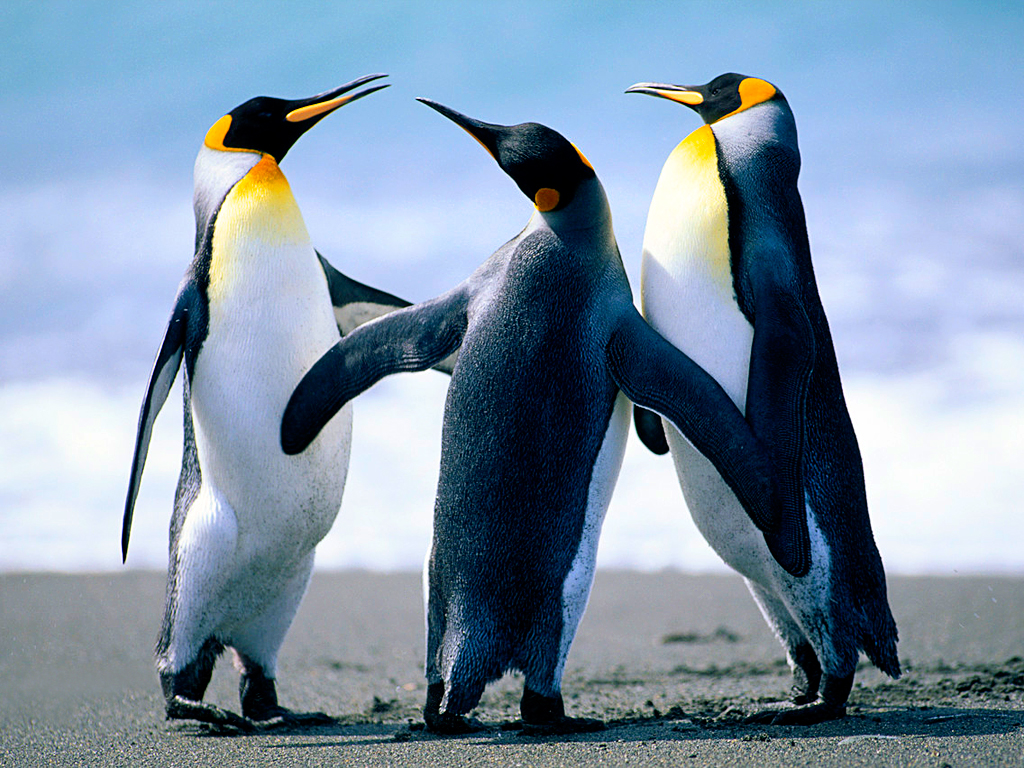
\includegraphics[scale=.50]{figures/Penguins.jpg}
\caption{TAMU figure - This is an example of a long figure title with a landscape figure.  Figure titles need to be single-spaced within and double spaced between in the list of figures.}
\label{fig:tamu-fig1-1}
\end{sidewaysfigure}
%%%%%%%%%%%%%%%%%%%%%%%%%%%%%%%%%%%%%%%%%%%%%%%%%%%%%%

More text here goes here.


Lorem ipsum dolor sit amet, consectetur adipiscing elit. Morbi augue urna, varius quis facilisis ac, imperdiet et nunc. Vestibulum ante ipsum primis in faucibus. 

\section{Testing the Top of the Page}
Maecenas accumsan lobortis dui fringilla suscipit. Quisque congue fringilla dui, sed eleifend sapien fringilla euismod. Pellentesque habitant morbi tristique senectus et netus et malesuada fames ac turpis egestas. Maecenas venenatis posuere magna quis tempus. Cras at leo massa, eu ultricies tellus. Nunc nec dictum augue. Cum sociis natoque penatibus et magnis dis parturient montes, nascetur ridiculus mus. Phasellus purus felis, mollis id scelerisque in, viverra in elit. Nulla iaculis ultrices justo, ac pharetra nisl rhoncus pulvinar. Duis vitae mauris velit, in congue massa.

Donec lectus orci, bibendum ut blandit dignissim, molestie non eros. Praesent aliquet feugiat dignissim. Morbi porttitor sollicitudin nisl, non mollis quam ultrices sit amet. Cras feugiat lacinia diam ut convallis. Nam nec varius ante. Nunc a ultrices felis. Quisque luctus sapien et ligula ornare quis consequat urna aliquet. Vestibulum vulputate lorem a tellus auctor id commodo risus sodales. Suspendisse quis tortor a felis molestie laoreet ut a nunc. Donec gravida sapien eget mauris condimentum lacinia. Proin eu purus libero. Nullam augue mi, vestibulum in convallis eu, adipiscing ac arcu. Donec nisi libero, egestas et molestie in, mollis quis ipsum. Sed gravida quam sit amet ante tempus rutrum non in mi. Cras viverra facilisis eros, id vestibulum sapien malesuada eget. Maecenas imperdiet luctus nisi vitae suscipit.



Aliquam erat volutpat. Integer ut mauris elit. Nam et lectus vel neque vehicula commodo. Integer at risus ligula. Fusce mollis mauris sed lorem aliquam bibendum porttitor tellus blandit. Curabitur enim nibh, accumsan eu elementum id, rutrum a ipsum. Vivamus ultricies, elit id ornare iaculis, metus justo posuere quam, sit amet bibendum arcu dolor a eros. Sed in nisl nibh. Aenean egestas est ut tortor volutpat vehicula. Maecenas aliquet placerat nunc hendrerit dictum. In et nisi massa. Pellentesque luctus, sapien quis dignissim vulputate, sapien libero bibendum velit, vitae auctor ipsum nulla at augue. Nulla ac eros vitae tortor elementum vehicula.

Morbi tristique egestas placerat. Cras faucibus eleifend porta. Class aptent taciti sociosqu ad litora torquent per conubia nostra, per inceptos himenaeos. Ut a pellentesque neque. Donec sollicitudin metus varius nulla egestas laoreet. Duis non mauris ut nunc adipiscing volutpat. Nam vitae est sed turpis tristique varius. 

\subsection{This is a Very Long Subsection Title This is a Very Long Subsection Title}

More text
\subsection{Subsection}

Subsection text

\section{Another Section}

Section text

%%%%%%%%%%%%%%%%%%%%%%%%%%%%%%%%%%%%%%%%%%%%%%%%%%%
%
%  New template code for TAMU Theses and Dissertations starting Fall 2012.  
%  For more info about this template or the 
%  TAMU LaTeX User's Group, see http://www.howdy.me/.
%
%  Author: Wendy Lynn Turner 
%	 Version 1.0 
%  Last updated 8/5/2012
%
%%%%%%%%%%%%%%%%%%%%%%%%%%%%%%%%%%%%%%%%%%%%%%%%%%%

%%%%%%%%%%%%%%%%%%%%%%%%%%%%%%%%%%%%%%%%%%%%%%%%%%%%%%%%%%%%%%%%%%%%%%%
%%%                           SECTION II
%%%%%%%%%%%%%%%%%%%%%%%%%%%%%%%%%%%%%%%%%%%%%%%%%%%%%%%%%%%%%%%%%%%%%%

\chapter{\uppercase {Literature Review: The Importance of Research Part Two- This is designed to test long titles in the TOC}}

Text goes here.

\section{New Section}
%%%%%%%%%%%%%%%%%%%%%%%%%%%%%%%%%%%%%%%%%%%%%%%%%%%%%%
\begin{figure}[H]
\centering
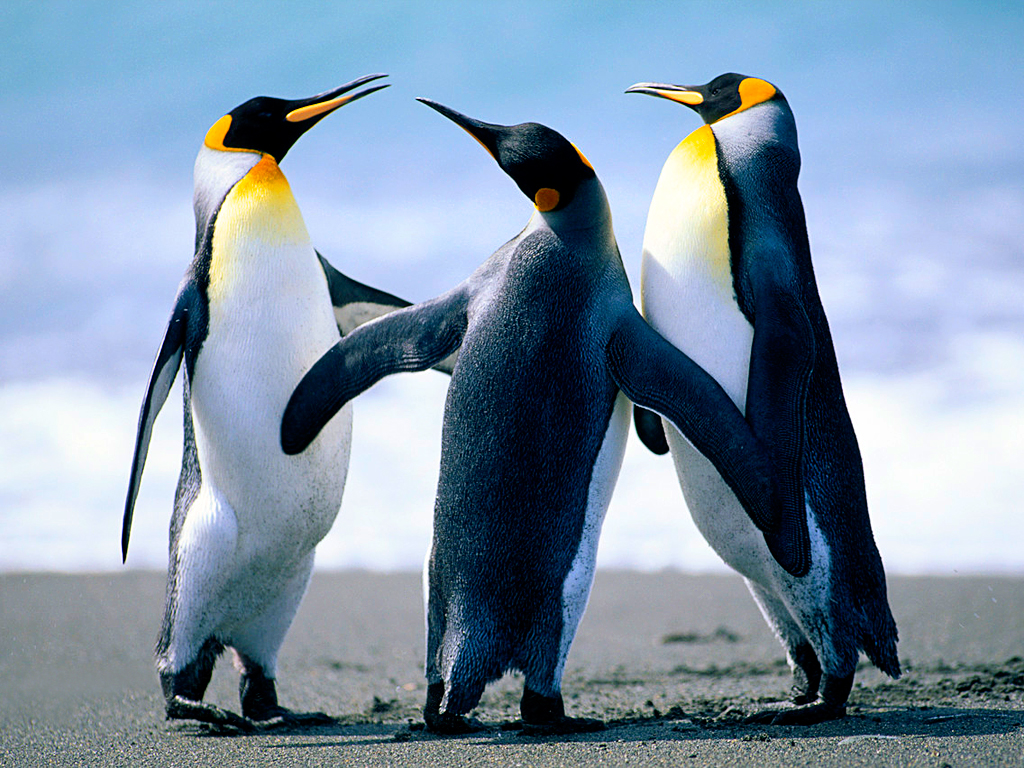
\includegraphics[scale=.50]{figures/Penguins.jpg}
\caption{TAMU figure - This is an example of a long figure title.  Figure titles need to be single-spaced within and double spaced between in the list of figures.}
\label{fig:landscapepenguins}
\end{figure}
%%%%%%%%%%%%%%%%%%%%%%%%%%%%%%%%%%%%%%%%%%%%%%%%%%%%%%
\subsection{Subsection}
\begin{table}[H]
\centering
\caption{This is a table template - This is an example of a long table title.  Table titles need to be single-spaced within and double spaced between in the list of tables.}
\begin{tabular}{|l|c|c|c|c|c|}
\hline
Product & 1 & 2 & 3 & 4 & 5\\
\hline
Price & 124.- & 136.- & 85.- & 156.- & 23.-\\
Guarantee [years] & 1 & 2 & - & 3 & 1\\
Rating & 89\% & 84\% & 51\% & & 45\%\\
\hline
\hline
Recommended & yes & yes & no & no & no\\
\hline
\end{tabular}
\label{tab:template1}
\end{table}


\subsection{Subsection}
%%%%%%%%%%%%%%%%%%%%%%%%%%%%%%%%%%%%%%%%%%%%%%%%%%%%%%
\begin{figure}[H]
\centering
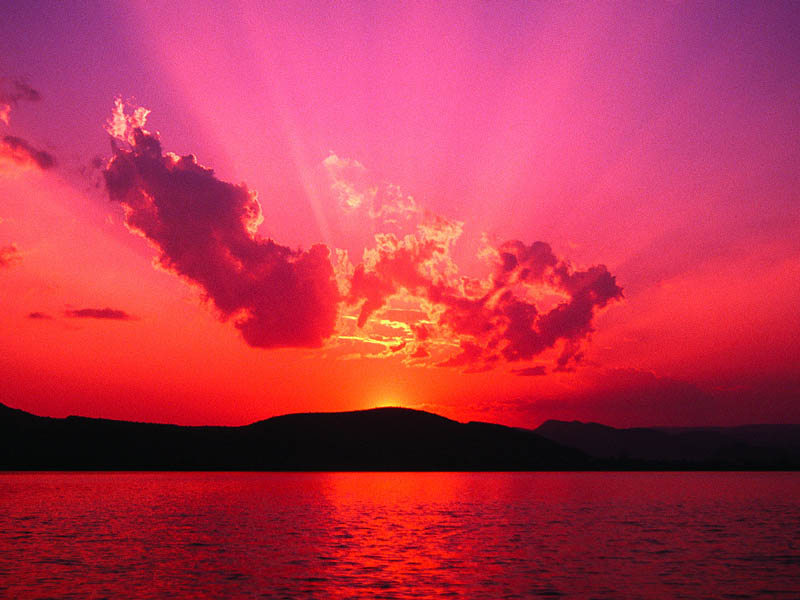
\includegraphics[scale=.50]{figures/Sunset.jpg}
\caption{Sunset figure}
\label{fig:sunset-fig2}
\end{figure}
%%%%%%%%%%%%%%%%%%%%%%%%%%%%%%%%%%%%%%%%%%%%%%%%%%%%%%
\subsubsection{This is a subsubsection}
\begin{table}[H]
\centering
\caption{This is a table template - This is an example of a long table title.  Table titles need to be single-spaced within and double spaced between in the list of tables.}
\begin{tabular}{|l|c|c|c|c|c|}
\hline
Product & 1 & 2 & 3 & 4 & 5\\
\hline
Price & 124.- & 136.- & 85.- & 156.- & 23.-\\
Guarantee [years] & 1 & 2 & - & 3 & 1\\
Rating & 89\% & 84\% & 51\% & & 45\%\\
\hline
\hline
Recommended & yes & yes & no & no & no\\
\hline
\end{tabular}
\label{tab:template1-2}
\end{table}
\section{Another Section}

%%%%%%%%%%%%%%%%%%%%%%%%%%%%%%%%%%%%%%%%%%%%%%%%%%%
%
%  New template code for TAMU Theses and Dissertations starting Fall 2012.  
%  For more info about this template or the 
%  TAMU LaTeX User's Group, see http://www.howdy.me/.
%
%  Author: Wendy Lynn Turner 
%	 Version 1.0 
%  Last updated 8/5/2012
%
%%%%%%%%%%%%%%%%%%%%%%%%%%%%%%%%%%%%%%%%%%%%%%%%%%%
%%%%%%%%%%%%%%%%%%%%%%%%%%%%%%%%%%%%%%%%%%%%%%%%%%%%%%%%%%%%%%%%%%%%%%
%%                           SECTION III
%%%%%%%%%%%%%%%%%%%%%%%%%%%%%%%%%%%%%%%%%%%%%%%%%%%%%%%%%%%%%%%%%%%%%



\chapter{\uppercase{Last Chapter: The Importance of Research}}

Text goes here \cite{Agrawal1986}.

\section{New Section}

%%%%%%%%%%%%%%%%%%%%%%%%%%%%%%%%%%%%%%%%%%%%%%%%%%%%%%
\begin{figure}[H]
\centering
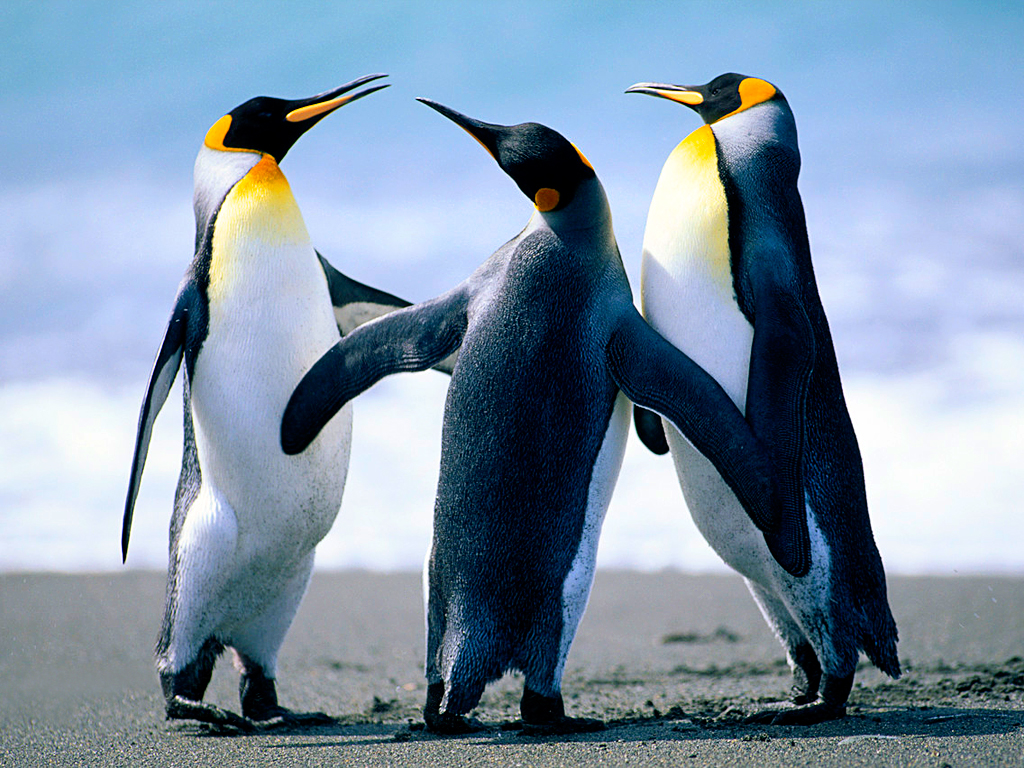
\includegraphics[scale=.50]{figures/Penguins.jpg}
\caption{TAMU figure}
\label{fig:tamu-fig3}
\end{figure}
%%%%%%%%%%%%%%%%%%%%%%%%%%%%%%%%%%%%%%%%%%%%%%%%%%%%%%
\section{Another Section}

Text between the figures.  Text between the figures. Text between the figures. Text between the figures.  Text between the figures. Text between the figures. Text between the figures.  Text between the figures. Text between the figures. Text between the figures.  Text between the figures. Text between the figures.
%%%%%%%%%%%%%%%%%%%%%%%%%%%%%%%%%%%%%%%%%%%%%%%%%%%%%%%
%\begin{figure}[H]
%\centering
%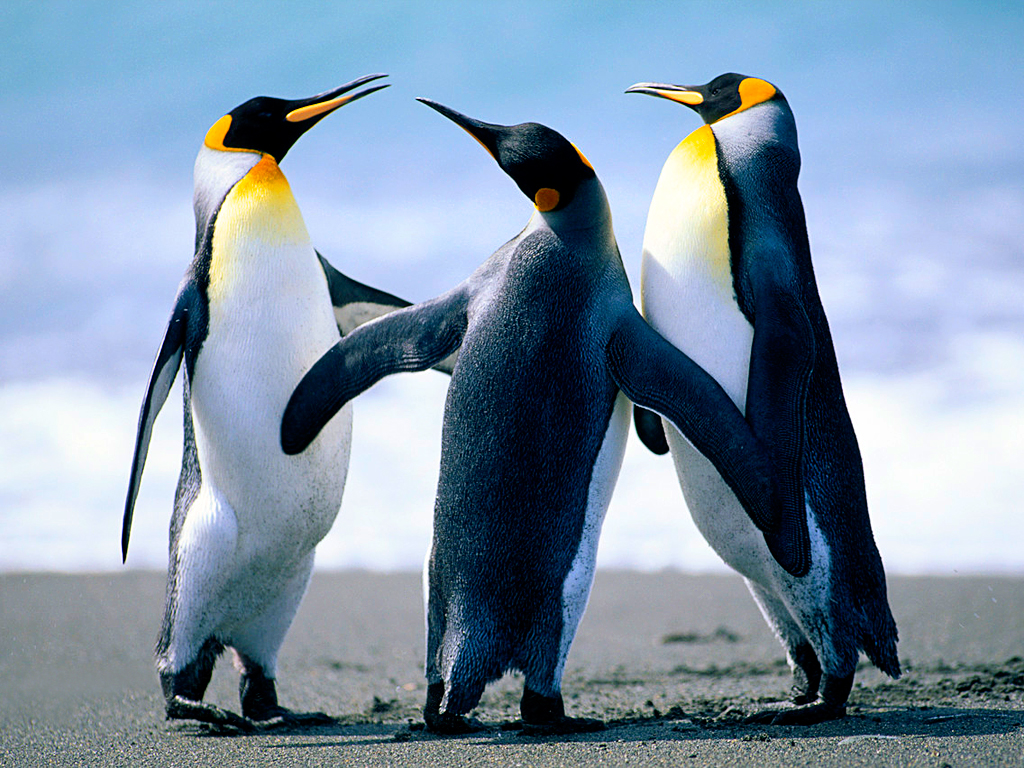
\includegraphics[scale=.50]{figures/Penguins.jpg}
%\caption{Another TAMU figure}
%\label{fig:tamu-fig4}
%\end{figure}
%%%%%%%%%%%%%%%%%%%%%%%%%%%%%%%%%%%%%%%%%%%%%%%%%%%%%%%

\subsection{Subsection}

%%%%%%%%%%%%%%%%%%%%%%%%%%%%%%%%%%%%%%%%%%%%%%%%%%%%%%%
%\begin{figure}[H]
%\centering
%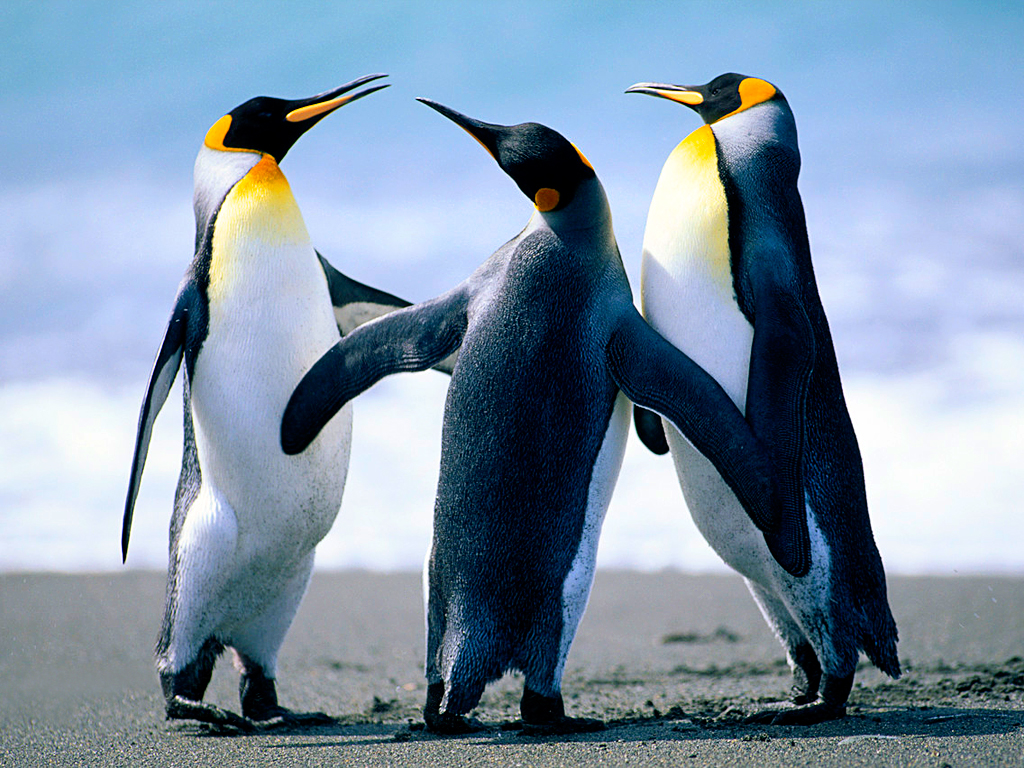
\includegraphics[scale=.50]{figures/Penguins.jpg}
%\caption{Another TAMU figure}
%\label{fig:tamu-fig4-2}
%\end{figure}
%%%%%%%%%%%%%%%%%%%%%%%%%%%%%%%%%%%%%%%%%%%%%%%%%%%%%%%
\subsection{Subsection}

A table example is going to follow.

\begin{table}[H]
\centering
\caption{This is a table template}
\begin{tabular}{|l|c|c|c|c|c|}
\hline
Product & 1 & 2 & 3 & 4 & 5\\
\hline
Price & 124.- & 136.- & 85.- & 156.- & 23.-\\
Guarantee [years] & 1 & 2 & - & 3 & 1\\
Rating & 89\% & 84\% & 51\% & & 45\%\\
\hline
\hline
Recommended & yes & yes & no & no & no\\
\hline
\end{tabular}
\label{tab:template2}
\end{table}
\subsubsection{This is a subsubsection}
\section{Another Section}

fix spacing in bibliography, if any...
%%%%%%%%%%%%%%%%%%%%%%%%%%%%%%%%%%%%%%%%%%%%%%%%%%%%%%%%%%%%%
\let\oldbibitem\bibitem
\renewcommand{\bibitem}{\setlength{\itemsep}{0pt}\oldbibitem}
%%%%%%%%%%%%%%%%%%%%%%%%%%%%%%%%%%%%%%%%%%%%%%%%%%%%%%%%%%%%%%%
%%%%%%%%%%%%%%%%%%%%%%%%%%%%%%%%%%%%%%%%%%%%%%%%%%%
%
%  New template code for TAMU Theses and Dissertations starting Fall 2012.  
%  For more info about this template or the 
%  TAMU LaTeX User's Group, see http://www.howdy.me/.
%
%  Author: Wendy Lynn Turner 
%	 Version 1.0 
%  Last updated 8/5/2012
%
%%%%%%%%%%%%%%%%%%%%%%%%%%%%%%%%%%%%%%%%%%%%%%%%%%%


%%%%%%%%%%%%%%%%%%%%%%%%%%%%%%%%%%%%%%%%%%%%%%%%%%%%%%%%%%%%%%%%%%%%%%
%%                           REFERENCES 
%%%%%%%%%%%%%%%%%%%%%%%%%%%%%%%%%%%%%%%%%%%%%%%%%%%%%%%%%%%%%%%%%%%%%

\phantomsection
\addcontentsline{toc}{chapter}{REFERENCES}

\renewcommand{\bibname}{{\normalsize\rm REFERENCES}}

\bibliographystyle{unsrt}
\bibliography{references}

%%%%%%%%%%%%%%%%%%%%%%%%%%%%%%%%%%%%%%%%%%%%%%%%%%%
%
%  New template code for TAMU Theses and Dissertations starting Fall 2012.  
%  For more info about this template or the 
%  TAMU LaTeX User's Group, see http://www.howdy.me/.
%
%  Author: Wendy Lynn Turner 
%	 Version 1.0 
%  Last updated 8/5/2012
%
%%%%%%%%%%%%%%%%%%%%%%%%%%%%%%%%%%%%%%%%%%%%%%%%%%%

\begin{appendices}
\titleformat{\chapter}{\centering\normalsize}{APPENDIX \thechapter}{0em}{\vskip .5\baselineskip\centering}
\renewcommand{\appendixname}{APPENDIX}

\addtocontents{toc}{\protect\renewcommand{\protect\cftchapaftersnum}{}}

%%%%%%%%%%%%%%%%%%%%%%%%%%%%%%%%%%%%%%%%%%%%%%%%%%%
%
%  New template code for TAMU Theses and Dissertations starting Fall 2012.  
%  For more info about this template or the 
%  TAMU LaTeX User's Group, see http://www.howdy.me/.
%
%  Author: Wendy Lynn Turner 
%	 Version 1.0 
%  Last updated 8/5/2012
%
%%%%%%%%%%%%%%%%%%%%%%%%%%%%%%%%%%%%%%%%%%%%%%%%%%%

%%%%%%%%%%%%%%%%%%%%%%%%%%%%%%%%%%%%%%%%%%%%%%%%%%%%%%%%%%%%%%%%%%%%%%
%%                           APPENDIX A 
%%%%%%%%%%%%%%%%%%%%%%%%%%%%%%%%%%%%%%%%%%%%%%%%%%%%%%%%%%%%%%%%%%%%%

\phantomsection

\chapter{\uppercase{Derivations and Equations for the LO System}}

\section{Useful Moment Relations for LO Equations}
\label{app:lo_mom_relations}

There are several relations between various moment definitions that are useful in
derivation and manipulation of the LO equations. The following are derived for $\phi(x)$,
but can be applied to general moments of functions.  The volumetric average terms
can be eliminated in terms of the $L$ and $R$ moments from the relation
$b_{L,i}(x)+b_{R,i}(x)=1$.
\begin{align}\label{app:atoL}
    \phi_{i} &= \frac{1}{h_i} \int\limits_\xl^\xr 1 \;\phi(x) \dd x \\
             &= \frac{1}{h_i} \left(\int\limits_\xl^\xr b_{L,i}(x) \phi(x) \dd x +
             \int\limits_\xl^\xr b_{R,i}(x) \phi(x) \dd x \right)\\
             &= \frac{1}{2} \left( \mom{\phi}_{L,i} + \mom{\phi}_{R,i} \right)
\end{align}
A similar relation can be derived for the first moment in space as
\begin{equation}
    {\phi}_{x,i} = \frac{3}{2} \left(\mom{\phi}_{R,i} - \mom{\phi}_{L,i}\right)
\end{equation}
The above relations can be inverted to derived a relation for the $L$ and $R$ moments in terms of the slope
and average moments.  These moment expressions are defined purely in terms of integrals,
and are independent of the chosen spatial representation

Once a linear relation on the interior has been assumed, there are other useful closures that can be
derived.  The standard linear interpolatory expansion, for the positive half-range, is restated here:
\begin{equation}
\phi^+(x) = \phi^+_{L,i} b_{L,i}(x) + \phi^+_{R,i} b_{R,i}(x)
\end{equation}
Using this expansion, one can derive a relation between the outflow from a cell and the
hat function moments that is equivalent to the standard LDFE Galerkin method:
\begin{equation}
    \phi_{i,R}^+ = 2 \mom{\phi}_{R,i}^+ - \mom{\phi}_{L,i}^+,
\end{equation}
where for standard LD $\phi_{i+1/2}^+\equiv\phi_{i,R}$.  The assumption of a linear relation on the interior
of the cell defines the value for $\phi_{i,L}^+$:
\begin{equation}
    \phi_{i,L}^+ = 2 \mom{\phi}_{L,i}^+ - \mom{\phi}_{R,i}^+,
\end{equation}

To eliminate the LO unknowns in a manner that produces the same moments as the LDFE
Galerkin method, the
following expression can be used for the outflow from a cell
\begin{equation}
    \phi_{i+1/2}^+ = \phi_i^+ + \frac{\phi_{x,i}^+}{3},
\end{equation}
which in terms of the hat function moments is equivalent to $\phi_{i+1/2}^+ =
\mom{\phi}_{R,i}^+$.  Inserting this expression into Eq.~\eqref{}, and using the same
definition for the linear representation over the interior of $\phi_{i+1/2}^+(x) =
\phi_{L,i} b_{L,i}(x) + \phi_{R,i} b_{R,i}(x)$, will produce an equivalent set of unknowns
as a linear discontinuous method with a lumped representation for the radiation.  The
temperature equation must be independently lumped. This
relation preserves the average within a cell but modifies the first moment.  

A similar expression produces a lumped-equivalent representation on the interior of the cell:
\begin{equation}
    \phi_{i,R}^+ = \phi_i^+ + \frac{\phi_x^+}{3},
\end{equation}
The moment equations are not modified by using this expression, however the interpretation
of the moments as a linear representation over the cell has been altered.  This allows for
us to ensure a lumped representation on the interior while still using the HO solution to
eliminate the outflow from the equations.


\section{Newtons Method for the LO Equations}
\label{app:lo_newton}

Because we have only considered problems with constant densities and heat capacities, the
linearization described below is in terms of temperature $T$ rather than material internal
energy, for simplicity. However, the linearization can be formed in terms of internal energy
to apply this method to a general equation of state.

To formulate the Newton iterations, the Planckian source is linearized in the material and radiation equations (Eq.~\eqref{??}
\& Eq.~\eqref{???}).
Application of the first order Taylor expansion in time to the
implicit emission source $B(T^{n+1})$, about some temperature $T^*$ at some
time $t^*\in[t^{n},t^{n+1}]$, yields
\begin{equation}\label{new_planck}
    \sigma_a^{n+1} a c T^{4,n+1} \simeq \sigma_a^* a c \left[T^{*4} + (T^{n+1} - T^*) 4T^{*3} \right]
\end{equation}
where $\sigma_a^*\equiv\sigma_a(T^*)$.  Substitution of this expression into Eq.~\eqref{eq:mat_cont} yields
\begin{equation}
    \rho c_v \left( \frac{T^{n+1} - T^{n}}{\Delta t} \right) = \sigma_a^* \phi^{n+1} -
    \sigma_a^* a c \left[ T^{*4} +  (T^{n+1} - T^*) 4T^{*3} \right].
\end{equation}
Algebraic manipulation of this equation yields an expression for $T^{n+1} - T^{*}$:
\begin{align*}
\left( T^{n+1} - T^* \right) &= \frac{ {\displaystyle \frac{\sigma_a^* \Delta t}{\rho
c_v}}  \left[ \phi^{n+1} -  a c T^{*4} \right] + (T^n - T^*) }{1 +
        \sigma_a^* a c \Delta t\frac{\displaystyle 4
T^{*3}}{\displaystyle \rho c_v } }.
\end{align*}
%This provides an expression for $T^{n+1}$ as a
%function of $T^*$ and the mean intensity $\phi^{n+1}$, i.e.,
%\begin{equation}
%\label{lo_t_new}
%T^{n+1}  = \frac{1}{\rho c_v } f\sigma_a^* \Delta t \left( \phi^{n+1} - c a T^{*4} \right)
%+ f T^n + (1-f) T^*.
%\end{equation}
This expression is substituted back into Eq.~\eqref{new_planck} to form
an explicit approximation for the emission source at $t^{n+1}$ as
\begin{equation}\label{t_next1}
    \sigma_a a c T^{4,n+1} \simeq \sigma_a^* (1 -f^*) \phi^{n+1}
    + f^* \sigma_a^* a c T^{4,n} + \rho c_v\frac{1-f^*}{\Delta t} (T^n - T^*)
\end{equation}
where $f^* = [1 + \sigma_a^* c \Delta t 4 a T^{*3}/(\rho c_v)]^{-1}$ is often referred to
as the Fleck factor~\cite{fnc}. 

Next, the above equation must be spatially discretized.  Application of the $L$ spatial
moment yields
\begin{multline}\label{eq:temp_const}
    \mom{\sigma_a^* a c T^{4,n+1}}_{L,i} = \sigma^*_{ai}(1-f_i^*)\mom{\phi^{n+1}}_{L,i} +
    f_i^*
    \sigma^*_{ai} a c \left(\frac{2}{3} T_{L,i}^{4,n} + \frac{1}{3} T_{R,i}^{4,n}\right)
    \\ \rho_i c_{vi} \frac{1 - f^*_i}{\Delta t} \left[\frac{2}{3}\left(T^n_{L,i} -
        T^*_{L,i}\right) + \frac{1}{3}\left(T^n_{R,i} -
    T^*_{R,i}\right)\right],
\end{multline}
where $T^{4,n}$ and $T^{n}$ have been assumed LD and $f^*$ is assumed constant over a cell, i.e., $f^*_i
\equiv \sigma_a(T_i^*)$.
The error introduced by a constant $f^*$ approaches zero as the
non-linearity is converged because $T^*$ approaches $T^{n+1}$. 
Based on an estimate for $T^*$, Eq.~\eqref{eq:temp_const} is an expression for
the Planckian emission source in the radiation moment equations with an additional effective scattering source.
A similar expression can be derived for $\mom{\sigma_{a,i} a c T^4}_R$ and the right
moment equations.
The expressions for the emissions source is substituted into the radiation moment equations
(Eq.~\eqref{eq:lo_tran}--~\eqref{???}) to produce a
linear system of equations for the new radiation intensity moments. 

Once the linear equations have been solved for new radiation moments, new temperature
unknowns can be estimated.  To conserve energy, the same linearization and discretizations used to
solve the radiation equation must be used in the material energy equation.
Substitution of Eq.~\eqref{eq:temp_const} into the material energy $L$ moment equation
ultimately yields
\begin{multline}\label{eq:new_temp}
    \frac{2}{3}T_{L,i}^{n+1} + \frac{1}{3}T_{R,i}^{n+1}= \frac{f_i^* \sigma_{ai}^* \Delta
t}{\rho c_{v}}  \left[ \mom{\phi^{n+1}}_{L,i}  - a c\left(\frac{2}{3} T_{L,i}^{4,n} + \frac{1}{3} T_{R,i}^{4,n}\right)
\right] + \\ (1- f^*_{i})\left(\frac{2}{3}T^*_{L,i} + \frac{1}{3}T^*_{R,i}\right) + f
\left(\frac{2}{3}T^n_{L,i} + \frac{1}{3}T^n_{R,i}\right)
\end{multline}
A similar expression is produced for the $R$ moment equation.  This produces a local
matrix equation to solve for new $T$ unknowns.  If both the radiation and temperature unknowns
are lumped, this matrix becomes diagonalized.

Based on these equations, the algorithm for solving the LO equations, with iteration index
$l$, is defined as
\begin{enumerate}
    \item Initialize $T$ unknowns using $T^n$ or the last estimate of $T^{n+1}$ from
        previous LO solve
    \item  Build the LO system based on the effective scattering $(1-f^l)$ and emission terms
          evaluated using $T^l$.
    \item Solve the linearized LO system to produce an estimate for $\phi^{n+1,l}$.
    \item Evaluate a new estimate of $T^{n+1}$ unknowns using Eq.~\eqref{eq:new_temp}.
    \item $T^*\leftarrow\tilde{T}^{n+1}$.
    \item Repeat 2-5 until $(T^{n+1,k})^4$ and $\phi^{n+1,k}$ are converged.
\end{enumerate}

\begin{figure}[H]
\centering
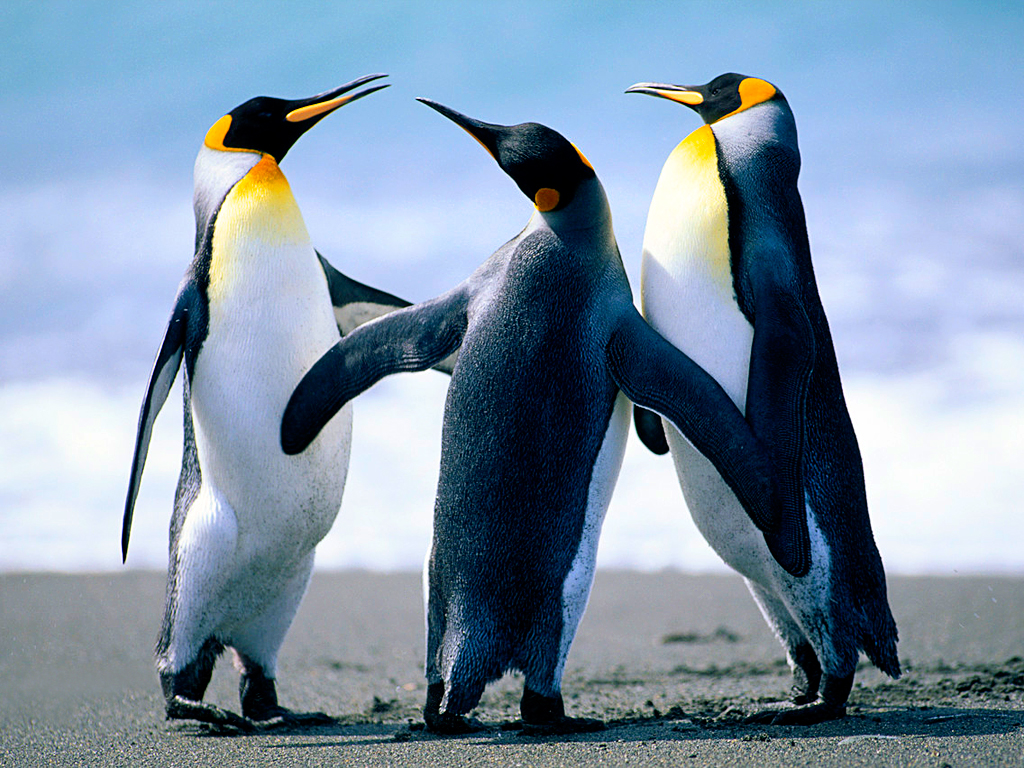
\includegraphics[scale=.50]{figures/Penguins.jpg}
\caption{TAMU figure}
\label{fig:tamu-fig5}
\end{figure}


\section{Analytic Neutronics answer for Source fixup}

In this section we model a fixed-source, pure-absorber neutronics calculation where we know the
analytic answer to test our fixup.  If we make the mesh thick enough, we can set the
solution to be the equilibrium answer $\psi(x) = \frac{q(x)}{2\sigma_a}$. For a general
isotropic source $Q(x)$, the 1D transport equation to be solved is
\begin{equation}
    \mu \pderiv{\psi}{x} + \sigma_a \psi(x,\mu) = \frac{q(x)}{2}
\end{equation}
with boundary condition $\psi(0,\mu)=\psi_{inc}$, $\mu>0$ and
$\psi(x_R,\mu)=\frac{q(x_R)}{2\sigma_a}$ for
$\mu<0$, where $x_R$ is the right boundary.  
This first order differential equation is solved using an integration factor.
The solution to this equation for $\mu>0$ is given by
\begin{equation}
    \psi(x,\mu) = \psi_{inc}e^{\frac{-\sigma_a x}{\mu}} + \int_0^x \frac{q(x')}{2\mu}
    e^{\frac{-\sigma_a x'}{\mu}} \dd x',\quad \mu>0
\end{equation}
Integration of this result over the positive half range of $\mu$ gives
\begin{equation}
    \phi^+(x) = \psi_{inc}\E2(\sigma_a x) + \frac{1}{2}\int_0^x q(x')\E1(\sigma_a x')
    \dd x'.
\end{equation}
In the simplification of a constant source, the integral reduces to
\begin{equation}
    \phi^+(x) = \psi_{inc}\E2(\sigma_a x) + \frac{q}{2\sigma_a} \left(1 -
    \E2(\sigma_ax)\right).
\end{equation}
Also, for a constant source the solution for the negative half range becomes a constant, i.e.,
\begin{equation}
    \phi^{-}(x) = \frac{q}{\sigma_a}
\end{equation}
Combination of the above two equations gives the solution for the scalar flux:
\begin{equation}
    \phi(x) = \psi_{inc}\E2(\sigma_a x) + \frac{q}{2\sigma_a} \left(1 -
    \E2(\sigma_ax)\right) + \frac{q}{\sigma_a}.
\end{equation}

\chapter{\uppercase{Derivation of the WLA-DSA Equations}}
\label{sec:wla_derivation}

In this section, we derive the discretized diffusion equation and LD mapping equations
that are used in the WLA-DSA equations.  To simplify notation, we
derive the equations from a generic transport equation (rather than the error equations) with isotropic scattering
and source $q_0$, i.e.,
\begin{equation}\label{eq:ss_trans}
    \mu \pderiv{I}{x} + \sigma_t I = \frac{\sigma_s}{2}\left( \phi(x) + q_0\right).
\end{equation}

\section{Forming a Continuous Diffusion Equation}

First, a continuous spatial discretization of a diffusion equation is derived.  
The mean intensity $\phi$ will ultimately be assumed continuous at faces to produce a
standard three-point finite-difference diffusion discretization. 
The zeroth and first $\mu$ moment of Eq.~\eqref{eq:ss_trans} produce the $P_1$
equations~\cite{lewis,wla_thesis}, i.e., 
\begin{align}\label{eq:dsa_bal}
    \pderiv{J}{x} + \sigma_a \phi &= q_0 \\ \label{eq:p1}
    \sigma_t J + \frac{1}{3} \pderiv{\phi}{x} &= 0.
\end{align}
The spatial finite element moments (defined by Eq.~\eqref{eq:x_moml} and~\eqref{x_momr})
are taken of the above equations. 
The mean intensity is assumed linear on the interior of the cell, i.e.,
$\phi(x)=\phi_Lb_L(x) + \phi_Rb_R(x)$, for $x\in(\xl,\xr)$.   Taking the left moment,
evaluating integrals, and rearranging yields
\begin{equation}
    J_{i} - J_{\il}  + \frac{\sigma_{a,i}h_i}{2} \left(\frac{2}{3} \phi_{L,i} + \frac{1}{3}
    \phi_{R,i} \right) = \frac{h_i}{2} \mom{q}_{L,i}\,\,,
\end{equation}
where $J_i$ is the average of the flux $J$ over the cell. The moments of $q$ are
not simplified to be compatible with the error equations which are in terms of moments. For the $R$ moment
\begin{equation}
    J_{i+1/2} - J_{i}  + \frac{\sigma_{a,i}h_i}{2} \left(\frac{2}{3} \phi_{L,i} + \frac{1}{3}
    \phi_{R,i} \right) = \frac{h_i}{2} \mom{q}_{R,i}\,\,.
\end{equation}
The equation for the $L$ moment is evaluated for cell $i+1$ and added to the $R$ moment
equation evaluated at $i$.  The flux $J$ is assumed continuous at $\ir$ to eliminate
the face fluxes from the equations.  The sum of the two equations becomes
\begin{multline}\label{eq:diff_noclose}
    J_{i+1} - J_{i} + \frac{\sigma_{a,i+1} h_{i+1}}{2}\left(\frac{2}{3} \phi_{L,i+1} +
    \frac{1}{3}\phi_{R,i+1}\right) + \frac{\sigma_{a,i} h_i}{2} \left( \frac{1}{3} \phi_{L,i} +
    \frac{2}{3}\phi_{R,i}\right) =\\ \frac{h}{2} \left(\mom{q}_{L,i+1} + \mom{q}_{R,i}
    \right).
\end{multline}
The mean intensity is approximated as continuous at each face, i.e., $\phi_{L,i+1} = \phi_{R,i}
\equiv \phi_{i+1/2}$.  Adding the $L$ and $R$ moments of Eq.~\eqref{eq:p1} together, with
the continuous approximation for $\phi_{i+1/2}$, produces a discrete Fick's law equation~\cite{stacy}
\begin{equation}\label{eq:ficks}
    J_{i} = -D_i \frac{\phi_{i+1/2} - \phi_{i-1/2}}{h_i},
\end{equation}
where $D_i = 1/(3\sigma_{t,i})$.
Substitution of Eq.~\eqref{eq:ficks} into Eq.~\eqref{eq:diff_noclose} and rearranging yields the following discrete diffusion
equation:
\begin{multline}
        \left(\frac{\sigma_{a,i+1} h_{i+1}}{6} -
        \frac{D_{i+1}}{h_{i+1}}\right)\phi_{i+3/2} + \left(\frac{D_{i+1}}{h_{i+1}} +
        \frac{D_{i}}{h_i} + \frac{\sigma_{a,i+1} h_{i+1}}{3} + \frac{\sigma_{a,i}
        h_{i}}{3}\right)\phi_{i+1/2} \\ + \left(\frac{\sigma_{a,i} h_{i}}{6} -
        \frac{D_{i}}{h_{i}}\right)\phi_{i-1/2} = \frac{h_{i+1}}{2} \mom{q}_{L,i+1} +
        \frac{h_{i}}{2}\mom{q}_{R,i}\;\,. 
\end{multline}
To allow for the use of lumped
or standard LD in these equations, we introduce the factor $\theta$, with
$\theta=1/3$ for standard
LD, and $\theta=1$ for lumped LD.  The diffusion equation becomes
\begin{multline}\label{eq:dsa_lumped}
    \left(\frac{\sigma_{a,i+1} h_{i+1}}{4}\left(1 - \theta\right)  -
        \frac{D_{i+1}}{h_{i+1}}\right)\phi_{i+3/2} + \left(\frac{D_{i+1}}{h_{i+1}} +
        \frac{D_{i}}{h_i} + \left(\frac{1+\theta}{2} \right)\left[\frac{\sigma_{a,i+1} h_{i+1}}{2} + \frac{\sigma_{a,i}
        h_{i}}{2}\right]\right)\phi_{i+1/2} \\ + \left(\frac{\sigma_{a,i}
        h_{i}}{4}\left(1 - \theta\right) -
        \frac{D_{i}}{h_{i}}\right)\phi_{i-1/2} = \frac{h_{i+1}}{2} \mom{q}_{L,i+1} +
        \frac{h_{i}}{2}\mom{q}_{R,i}
        \;\,. 
\end{multline}
Summation over all cells forms a system of equations for $\phi$ at each face.  

\subsection{Diffusion Boundary Conditions}

The upwinding in the LO system exactly satisfies the inflow boundary conditions, therefore
a vacuum boundary condition is applied to the diffusion error equations.  The equation for the left moment
at the first cell is given by
\begin{equation}\label{eq:dsa_bc_app}
    J_{1} - J_{1/2}  + \frac{\sigma_{a,i}h_i}{2} \left(\frac{1+\theta}{2} \phi_{L,i}
    + \frac{1-\theta}{2}
    \phi_{R,i} \right) = \frac{h_i}{2} \mom{q}_{L,i}\,\,,
\end{equation}
The Marshak boundary condition for the vacuum inflow at face $x_{1/2}$ is given as
\begin{equation}
    J^+_{1/2} = 0 = \frac{\phi_{1/2}}{4} + \frac{J_{1/2}}{2},
\end{equation}
which can be solved for $J_{1/2}$.  Substitution of the above equation and
Eq.~\eqref{eq:ficks} into Eq.~\eqref{eq:dsa_bc_app} gives 
\begin{equation}\label{eq:bc_dsa}
    \left(\frac{1}{2}+ \sigma_{a,1}h_1\frac{1+\theta}{4} - \frac{D_1}{h_1}\right)\phi_{1/2} +
    \left( {\sigma_{a,1}{h_1}}\frac{1-\theta}{4} - \frac{D_1}{h_1}  \right)\phi_{3/2} =
    \frac{h_i}{2} \mom{q}_{L,1}
\end{equation}
A similar expression can be derived for the right-most cell.

\section{Mapping Solution onto LD Unknowns}

Solution of the continuous diffusion equation will provide an approximation to $\phi$ on
faces, denoted as $\phi_{i+1/2}^C$. We now need to map the face solution onto 
the LD representation of $\phi$. To do this, first we take the $L$ and $R$ finite element moments of the P$_1$
equations.  A LDFE dependence is assumed on the interior of the cell for $J$ and
$\phi$.  Taking moments of Eq.~\eqref{eq:dsa_bal} and simplifying yields
\begin{align}
    J_{\ir} - \frac{J_{L,i} + J_{R,i}}{2} + \frac{\sigma_{a,i} h_i}{2} \left(\frac{1}{3} \phi_{L,i} +
    \frac{2}{3}\phi_{R,i}\right) &= \frac{h_i}{2} \mom{q}_{R,i} \\
    \frac{J_{L,i} + J_{R,i}}{2} - J_{i-1/2} + \frac{\sigma_{a,i} h_i}{2}
    \left(\frac{2}{3} \phi_{L,i} +
    \frac{1}{3}\phi_{R,i}\right) &= \frac{h_i}{2} \mom{q}_{L,i}
\end{align}
The moment equations for Eq.~\eqref{eq:p1} are
\begin{align}
    \frac{1}{3}\left(\phi_{\ir} - \frac{\phi_{i,L} + \phi_{i,R}}{2}\right) +
    \frac{\sigma_{t,i} h_i}{2} \left(\frac{1}{3} J_{L,i} + \frac{2}{3}J_{R,i}\right)
    &= 0 \\
    \frac{1}{3}\left(\frac{\phi_{i,L} + \phi_{i,R}}{2} - \phi_{i-1/2} \right) +
    \frac{\sigma_{t,i} h_i}{2} \left(\frac{2}{3} J_{L,i} + \frac{1}{3}J_{R,i}\right)
    &= 0 
\end{align}

The face terms $J_{i\pm 1/2}$ and $\phi_{i\pm 1/2}$ need to be eliminated from the
system. First, the scalar intensity is assumed to be the value provided by the continuous
diffusion solution at each face, i.e., $\phi_{i\pm1/2} = \phi_{i\pm1/2}^C$.
Then, the fluxes are decomposed into half-range values to decouple the equations
between cells.  At $x_{\ir}$, the flux is composed as $J_{i+1/2} = J_{\ir}^+ + J_{\ir}^-$,
noting that in this notation the half-range fluxes are $J_{\ir}^{\pm}=\pm \int_{0}^\pm
\mu I(x_{i+1/2},\mu) \dd \mu$\footnote{Typically, the half-range fluxes are defined with
    integrals weighted with $| \mu |$, but this notation would not be consistent with our
definition of the half-range consistency terms}.  We approximate the incoming fluxes, e.g.,
$J_{i+1/2}^-$, based on $\phi_{i+1/2}^C$ and a P$_1$ approximation.   
The P$_1$ approximation provides the following relation~\cite{wla_thesis}
\begin{equation}
    \phi = 2(J^+ - J^-).
\end{equation}
At $\xr$, the above expression is solved for the incoming current $J_{i+1/2}^-$.  The
total current becomes
\begin{equation}\label{eq:jelim}
    J_{\ir} = J_{\ir}^+ - J_{\ir}^- = 2J_{\ir}^+ - \frac{\phi_{i+1/2}^C}{2},
\end{equation}
In the positive direction, at the right face, the
values of $\phi$ and $J$ are based on the LD representation within the cell at that
face, i.e., $\phi_{R,i}$ and $J_{R,i}$.  The standard P$_1$ approximation for the
half-range fluxes is used\cite{stacy}, i.e.,
\begin{align}
    J^{\pm} &= \frac{\gamma \phi}{2} \pm \frac{J}{2},
\end{align}
where $\gamma$ accounts for the difference between the LO parameters and the true
P$_1$ approximation. Thus, for the right face and positive half-range,
\begin{align}
    J_{\ir}^+ &= \frac{\gamma}{2}\phi_{i,R} + \frac{J_{i,R}}{2} 
\end{align}
A similar expression can be derived for $\xl$.  The total fluxes at each face are
thus
\begin{align}
    J_{i+1/2} &= \gamma\phi_{i,R} + J_{i,R} - \frac{\phi_{\ir}^C}{2} \\
    J_{i-1/2} &= \frac{\phi_{i-1/2}^C}{2} - \gamma \phi_{i,L} + J_{i,L}
\end{align}
Substitution of these results back into the LD balance equations and introduction of the
lumping notation yields the final equations 
\begin{align}\label{eq:update1}
    \left(\gamma\phi_{i,R} + J_{i,R} - \frac{\phi_{\ir}^C}{2} \right) - \frac{J_{L,i} + J_{R,i}}{2} + \frac{\sigma_{a,i} h_i}{2} \left(
    \frac{(1-\theta)}{2} \phi_{L,i} +
    \frac{(1+\theta)}{2}\phi_{R,i}\right) &= \frac{h_i}{2} \mom{q}_{R,i} \\
    \frac{J_{L,i} + J_{R,i}}{2} -\left(\frac{\phi_{i-1/2}^C}{2} - \gamma \phi_{i,L} +
    J_{i,L}\right) + \frac{\sigma_{a,i} h_i}{2} \left(
    \frac{(1+\theta)}{2} \phi_{L,i} +
    \frac{(1-\theta)}{2}\phi_{R,i}\right) &= \frac{h_i}{2} \mom{q}_{L,i} 
    \\
    \frac{1}{3}\left(\phi_{i+1/2}^C - \frac{\phi_{i,L} + \phi_{i,R}}{2}\right) +
    \frac{\sigma_{t,i} h_i}{2}\left( \frac{(1-\theta)}{2} J_{L,i} +
    \frac{(1+\theta)}{2}J_{R,i}\right)    &= 0 \\
    \frac{1}{3}\left(\frac{\phi_{i,L} + \phi_{i,R}}{2} - \phi^C_{i-1/2} \right) +
    \frac{\sigma_{t,i} h_i}{2} \left( \frac{(1+\theta)}{2} J_{L,i} +
    \frac{(1-\theta)}{2}J_{R,i}\right) &= 0 . \label{eq:update2}
\end{align}
The above equations are completely local to each cell and fully defined, including for
boundary cells. For simplicity, we just take $\gamma=1/2$.  The system can be solved for the desired unknowns
$\phi_{i,L}$, $\phi_{i,R}$, $J_{i,L}$, and $J_{i,R}$, which represent the mapping of
$\phi_{i+1/2}^C$ onto the LD representation for $\phi^{\pm}(x)$.




\end{appendices}



\end{document}
